\chapter{Previous work}\label{previous_work}

\figref{geomod_interface} shows the main window for geometry visualization in GeoMod. Most of the work that has been done in GeoMod is concerned with generating 3D views of robots and trajectory planning. It also has the ability to calculate required motor torques and joint moments for static loads. The following chapter will shortly describe how this is done. 

\begin{figure}
 \centering 
 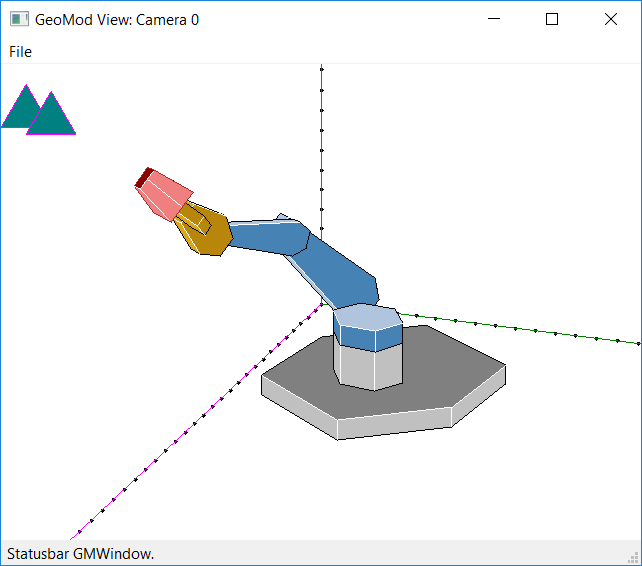
\includegraphics[width=.5\linewidth]{geomod_robot}
 \caption{GeoMod 3D visualization interface}
 \label{geomod_interface}
\end{figure}

\section{T-group}


The \texttt{Tgroup} class is a central part of the GeoMod program. A simplified version of the class can be seen in \liref{Tgroup}. Tgroup stands for transformation group and holds a collection of central parameters for a part, like center of gravity (line 3) and a combined position orientation (line 4). The latter is called extended basis in GeoMod but defined as a \textit{frame} in the theory at page \pageref{secTheory}. It also holds a list of coordinates for the geometry (line 7).

\lstinputlisting[caption={\texttt{tgroup.h}, simplified version}]{./snippet/Tgroup.h}\label{Tgroup}

%\lstinputlisting[caption={\texttt{extbas.h}, simplified version}]{./snippet/ExtBasis.h}\label{ExtBasis}

\vspace{-0.5cm}

\section{Kinematics}

A chained robot is made up of multiple parts described by the class \texttt{Part}, \liref{Part}. These parts could be the different parts of the chained robot in \figref{geomod_interface}. Each of the parts can be rotated with \glsf{dirkin}\textit{s} (line 9). The \glsf{invkin} is calculated geometrically by \texttt{invKin()}, meaning that the solution is found by a series of predefined geometric rules. These angles are then sent to \texttt{dirKin()} to perform the \gls{dirkin} movements. The last two functions are not part of the \texttt{Tgroup} or \texttt{Part} class.

\lstinputlisting[caption={\texttt{part.h}, simplified version}]{./snippet/Part.h}\label{Part}

\section{Dynamics}

\figref{geoMod_forces} shows the robot in GeoMod with joint moments visualized as arrows. The necessary motor torque (red) is calculated by taking the vector product of a radius and force vector for each joint. This calculation is performed after a direct or inverse kinematic movement has been done. No time-dependent variables or time itself is stored. This means that the calculations are purely static, no dynamic calculations are performed.

\begin{figure}[h!]
    \centering
    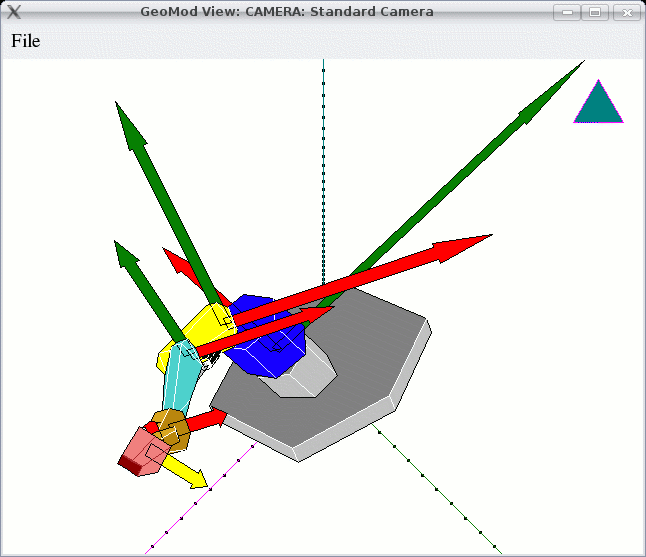
\includegraphics[width=.7\textwidth]{geoMod_forces}
    \caption{GeoMod graphics view showing moments acting on joints.}
    \label{geoMod_forces}
\end{figure}

To perform any dynamic calculations there are a few changes that had to be implemented during this project. First, the class structure had to store the exact time when calculations were performed. This way approximations to derivatives for various variables could be found. Secondly, movement had to be defined over a time interval so that definite values of velocity and acceleration could be calculated. This would also provide animation to the movement.

